\documentclass[11pt,letterpaper,boxed]{../hmcpset}
\usepackage[margin=1in]{geometry}
\usepackage{graphicx}
\usepackage{enumerate}
\usepackage{amsthm}
\usepackage{amsmath}

\newcommand{\ds}{\displaystyle}
\newcommand{\half}{\frac{1}{2}}
\newcommand*\Eval[3]{\left.#1\right\rvert_{#2}^{#3}}
\newcommand{\eval}{\biggr\rvert}
\newcommand\Partial[2]{\frac{\partial #1}{\partial #2}}
\renewcommand{\vec}[1]{\mathbf{#1}}
\def\EE{{\cal E}}
\def\Lagr{\mathcal{L}}


\name{}
\class{Physics 111 Section 1}
\assignment{Problem Set 03}
\duedate{September 12, 2016}

\begin{document}

\problemlist{The Lagrangian, Constrained Systems (Reading: Chapter 7.2--7.5)}
\textbf{Help:}

\begin{problem}[i]
Modify Lagrange's equations for a 1D~system with a non-conservative contraint force such as friction. 
In this case, which forces are included in the definition of $U(x)$? 
This is a straightforward problem, don't over think it.

\begin{problem}[7.12] 
Lagrange's equations in the form discussed in this chapter hold only if the forces (at least the nonconstraint forces) are derivable from a potential energy. 
To get an idea how they can be modified to include forces like friction, consider the following: 
A single particle in one dimension is subject to various conservative forces (net conservative force$= F = - \partial U / \partial x$) and a nonconservative force (let's call it $F_\text{fric}$). 
Define the Lagrangian as $\mathcal{L} = T - U$ and show that the appropriate modification is 
  \[ \frac{\partial \mathcal{L}}{\partial x} + F_\text{fric} = \frac{d}{dt} \frac{\partial \mathcal{L}}{\partial \dot x} \]
\end{problem}
\end{problem}

\begin{solution}

\vfill
\end{solution}

\newpage 

\begin{problem}[ii]
Prove that Lagrange's equations hold for two particles moving under unspecified constraints. 

\begin{problem}[7.13]
In Section~7.4 [Equations~(7.41 through (7.51)], I proved Lagrange's equations for a single particle constrained to move on a two-dimensional surface. 
Go through the same steps to prove Lagrange's equations for a system consisting of two particles subject to various unspecified constraints. 

\bigskip

[\textit{Hint}: The net force on particle~1 is the sum of the total constraint force $\vec{F}_1^\text{cstr}$ and the total nonconstraint force $\vec{F}_1$, and likewise for particle~2. 
The constraint forces come in many guises (the normal force of a surface, the tension force of a string tied between the particles, etc.), but it is always true that the net work done by all constraint forces in any displacement consistent with the constraints is zero---this is the defining property of constraint forces. 
Meanwhile, we take for granted that the nonconstraint forces are derivable from a potential energy $U(\vec{r}_1, \vec{r}_2, t)$; that is $\vec{F}_1 = - \nabla_1 U$ and likewise for particle~2. 
Write down the difference $\delta S$  between the action integral for the right path given by $\vec{r}_1(t)$ and $\vec{r}_2(t)$ and any nearby wrong path given by $\vec{r}_1(t) + \boldsymbol{\epsilon}_1(t)$ and $\vec{r}_2(t) + \boldsymbol{\epsilon}_2(t)$. 
Paralleling the steps of Section~7.4, you can show that $\delta S$ is given by an integral analogous to (7.49), and this is zero by the defining property of constraint forces.]
\end{problem}
\end{problem}

\begin{solution}

\vfill
\end{solution}

\newpage 

\begin{problem}[iii] 
An oscillating bead on a spinning hoop. 
Getting the correct expression for the velocity of the bead is tricky; keep in mind that while $\omega$ is constant, $\phi = \phi(t)$. 

\begin{problem}[7.35]
Figure~7.16 is a bird's-eye view of a smooth horizontal wire hoop that is forced to rotate at a fixed angular velocity $\omega$ about a vertical axis through the point $A$. 
A bead of mass $m$ is threaded on the hoop and is free to move around it, with its position specified by the angle $\phi$ that it makes at the center with the diameter $AB$. 
Find the Lagrangian for this system using $\phi$ as your generalised coordinate. 
(Read the hint in Problem~7.29.)
Use the Lagrange equation of motion to show that the bead oscillates about the point $B$ exactly like a simple pendulum. 
What is the frequency of these oscillations if their amplitude is small?
\[	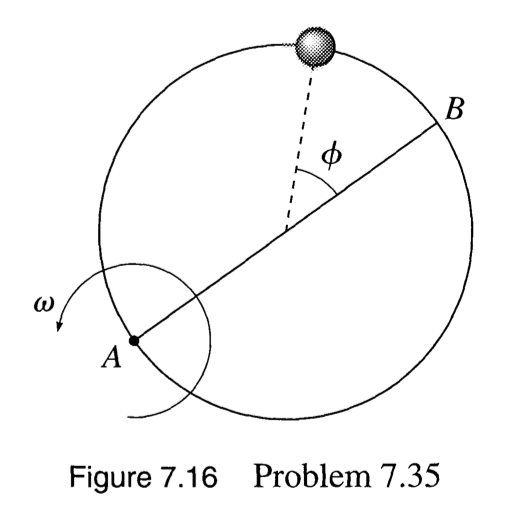
\includegraphics[scale=0.7]{fig1}\]
\end{problem}
\end{problem}

\begin{solution}
\vfill
\end{solution}

\newpage 

\begin{problem}[iv] 
A central force potential. In part~(c) focus on the $\theta$~equation and the type of motion it implies, and in part~(d) do the same thing but for your $\phi$~equation. 

\begin{problem}[7.39]
\begin{enumerate}[(a)]
\item Write down the Lagrangian for a particle moving in three dimensions under the influence of a conservative force with potential energy $U(r)$, using spherical polar coordinates $(r, \theta, \phi)$. 

\item Write down the three Lagrange equations and explain their significance in terms of radial acceleration, angular momentum, and so forth. 
(The $\theta$ equation is the tricky one, since you will find it implies that the $\phi$ component of $\boldsymbol{\ell}$ varies with time, which seems to contradict conservation of angular momentum. 
Remember, however that $\ell_\phi$ is the component of $\boldsymbol{\ell}$ in a \textit{variable} direction.)

\item Suppose that initially the motion is in the equatorial plane (that is, $\theta_0 = \pi/2$ and ${\dot \theta}_0 = 0$). 
Describe the subsequent motion. 

\item Suppose instead that the initial motion is along a line of longitude (that is, ${\dot \phi}_0 = 0$). 
Describe the subsequent motion. 
\end{enumerate}
\end{problem}
\end{problem}

\begin{solution}
\vfill
\end{solution}

\newpage 

\end{document}
